\appendix
\addtocontents{toc}{%
  \protect\vspace{1em}% 
  \protect\noindent \bfseries \appendixtocname\protect\par
  \protect\vspace{-.5em}%
 }
 \renewcommand{\chaptername}{\appendixname}
 
\begin{appendices}

\chapter{Appendix A}

\section{Application Script} \label{app:app_js}
\begin{lstlisting}[caption={app.js in application client},label={code:app_js}]
'use strict';

// Declare app level module which depends on filters, and services

angular.module('webrtcDemo', [
  'ui.bootstrap',
  'btford.socket-io',
  'angularLocalStorage',
  'angular-underscore',
  'ngRoute',
  'ui.keypress',
  'angularMoment',
  'angularFileUpload',
  'angular-table',
  'angucomplete-alt',
  'webrtcDemo.services.values',
  'webrtcDemo.services',
  'webrtcDemo.controllers',
  'webrtcDemo.directives',
  'webrtcDemo.filters'
]).
config(function ($routeProvider, $locationProvider, $httpProvider) {
  $routeProvider.
    when('/chat', {
      templateUrl: 'partials/phoneView',
      controller: 'PhoneViewCtrl'
    }).
    when('/login',{
      templateUrl: 'partials/login',
      controller: 'LoginViewCtrl'
    }).
    otherwise({
      redirectTo: '/login'
    });

  $locationProvider.html5Mode(true);

  $httpProvider.defaults.useXdomain = true;
  delete $httpProvider.defaults.headers.common['X-Requested-With'];
  $httpProvider.defaults.withCredentials = true;
});

angular.module('webrtcDemo.services', ['webrtcDemo.services.values']);

angular.module('webrtcDemo.controllers',['webrtcDemo.services.values']);

angular.module('webrtcDemo.directives',['webrtcDemo.services.values']);

angular.module('webrtcDemo.filters',['webrtcDemo.services.values']);
\end{lstlisting}

\section{WebRTCService Script} \label{app:webrtc_service}

\begin{lstlisting}[caption={WebRTCService.js in application client},label={code:webrtc_service}]
'use strict';

/**
*  services Module
*
* WebRTCService with browser adapter.js function
*/

angular.module('webrtcDemo.services').
	factory('WebRTCService',function () {
		var _ws;//websocket obj
		
		var _RTCPeerConnection;
		var _RTCSessionDescription;
		var _RTCIceCandidate;
		var _getUserMedia;
		var _createIceServer;
		var _attachMediaStream;
		var _reattachMediaStream;
		var _webrtcDetectedBrowser;
		var _webrtcDetectedVersion;

		function _initWebRTC () {
			_RTCPeerConnection = null;
			_RTCSessionDescription = null;
			_RTCIceCandidate = null;
			_getUserMedia = null;
			_createIceServer = null;
			_attachMediaStream = null;
			_reattachMediaStream = null;
			_webrtcDetectedBrowser = null;
			_webrtcDetectedVersion = null;

			_setRTCElement();
		}

		function _setRTCElement() {

			if(navigator.mozGetUserMedia){
				console.log("This appears to be Firefox");

				_webrtcDetectedBrowser = "firefox";
				_webrtcDetectedVersion = parseInt(navigator.userAgent.match(/Firefox\/([0-9]+)\./)[1], 10);

				_RTCPeerConnection = mozRTCPeerConnection;
				_RTCSessionDescription = mozRTCSessionDescription;
  			_RTCIceCandidate = mozRTCIceCandidate;
  			_getUserMedia = navigator.mozGetUserMedia.bind(navigator);

  			// Creates iceServer from the url for FF.
			  _createIceServer = function(url, username, password) {
			    var iceServer = null;
			    var url_parts = url.split(':');
			    if (url_parts[0].indexOf('stun') === 0) {
			      // Create iceServer with stun url.
			      iceServer = { 'url': url };
			    } else if (url_parts[0].indexOf('turn') === 0) {
			      if (_webrtcDetectedVersion < 27) {
			        // Create iceServer with turn url.
			        // Ignore the transport parameter from TURN url for FF version <=27.
			        var turn_url_parts = url.split("?");
			        // Return null for createIceServer if transport=tcp.
			        if (turn_url_parts.length === 1 ||
			            turn_url_parts[1].indexOf('transport=udp') === 0) {
			          iceServer = { 'url': turn_url_parts[0],
			                        'credential': password,
			                        'username': username };
			        }
			      } else {
			        // FF 27 and above supports transport parameters in TURN url,
			        // So passing in the full url to create iceServer.
			        iceServer = { 'url': url,
			                      'credential': password,
			                      'username': username };
			      }
			    }
			    return iceServer;
			  };

  			_attachMediaStream = function(element, stream) {
			    console.log("Attaching media stream");
			    element.mozSrcObject = stream;
			    element.play();
			  };

			  _reattachMediaStream = function(to, from) {
			    console.log("Reattaching media stream");
			    to.mozSrcObject = from.mozSrcObject;
			    to.play();
			  };

			  // Fake get{Video,Audio}Tracks
			  if (!MediaStream.prototype.getVideoTracks) {
			    MediaStream.prototype.getVideoTracks = function() {
			      return [];
			    };
			  }

			  if (!MediaStream.prototype.getAudioTracks) {
			    MediaStream.prototype.getAudioTracks = function() {
			      return [];
			    };
			  }

			}else if(navigator.webkitGetUserMedia){
				console.log("This appears to be Chrome");

				_webrtcDetectedBrowser = "chrome";
				_webrtcDetectedVersion = parseInt(navigator.userAgent.match(/Chrom(e|ium)\/([0-9]+)\./)[2], 10);

			  _RTCPeerConnection = webkitRTCPeerConnection;
			  _RTCSessionDescription = RTCSessionDescription;
			  _RTCIceCandidate = RTCIceCandidate;
			  _getUserMedia = navigator.webkitGetUserMedia.bind(navigator);

			  // Creates iceServer from the url for Chrome.
			  _createIceServer = function(url, username, password) {
			    var iceServer = null;
			    var url_parts = url.split(':');
			    if (url_parts[0].indexOf('stun') === 0) {
			      // Create iceServer with stun url.
			      iceServer = { 'url': url };
			    } else if (url_parts[0].indexOf('turn') === 0) {
			      if (_webrtcDetectedVersion < 28) {
			        // For pre-M28 chrome versions use old TURN format.
			        var url_turn_parts = url.split("turn:");
			        iceServer = { 'url': 'turn:' + username + '@' + url_turn_parts[1],
			                      'credential': password };
			      } else {
			        // For Chrome M28 & above use new TURN format.
			        iceServer = { 'url': url,
			                      'credential': password,
			                      'username': username };
			      }
			    }
			    return iceServer;
			  };

			  // Attach a media stream to an element.
			  _attachMediaStream = function(element, stream) {
			    if (typeof element.srcObject !== 'undefined') {
			      element.srcObject = stream;
			    } else if (typeof element.mozSrcObject !== 'undefined') {
			      element.mozSrcObject = stream;
			    } else if (typeof element.src !== 'undefined') {
			      element.src = URL.createObjectURL(stream);
			    } else {
			      console.log('Error attaching stream to element.');
			    }
			  };

			  _reattachMediaStream = function(to, from) {
			    to.src = from.src;
			  };

			  // The representation of tracks in a stream is changed in M26
			  // Unify them for earlier Chrome versions in the coexisting period
			  if (!webkitMediaStream.prototype.getVideoTracks) {
			    webkitMediaStream.prototype.getVideoTracks = function() {
			      return this.videoTracks;
			    };
			    webkitMediaStream.prototype.getAudioTracks = function() {
			      return this.audioTracks;
			    };
			  }

			  // New syntax of getXXXStreams method in M26
			  if (!webkitRTCPeerConnection.prototype.getLocalStreams) {
			    webkitRTCPeerConnection.prototype.getLocalStreams = function() {
			      return this.localStreams;
			    };
			    webkitRTCPeerConnection.prototype.getRemoteStreams = function() {
			      return this.remoteStreams;
			    };
			  }

			}else{
				console.log("Browser does not appear to be WebRTC-capable");
			}

		}

		return {
			init : function (socket) {
				if(socket){
					//init service with websocket
					_ws = socket;
				}

				_initWebRTC();

			},

			peerConnection : function(config,constraints){
				if(_RTCPeerConnection){
					return new _RTCPeerConnection(config,constraints);
				}
				return null;
			},

			RTCSessionDescription : function(message){
				if(_RTCSessionDescription){
					return new _RTCSessionDescription(message);
				}
				return null;
			},

			RTCIceCandidate : function(options){
				if(_RTCIceCandidate){
						return new _RTCIceCandidate(options);
					}
					return null;
			},

			webrtcDetectedBrowser : function(){
				return _webrtcDetectedBrowser;
			},

			attachMediaStream : function(element, stream){
				return _attachMediaStream(element, stream);
			},

			reattachMediaStream : function(to, from){
				return _reattachMediaStream(to, from);
			},

			getUserMedia : function(constraints, handleUserMedia, handleUserMediaError){
				return _getUserMedia(constraints, handleUserMedia, handleUserMediaError);
			}

		}
	});	
	
\end{lstlisting}

\section{ContactTable Scrtips} \label{app:contact_table}

\begin{lstlisting}[caption={contactTable.jade in application client},label={code:contact_table}]
div(id = "contactTable")
	angucomplete-alt(id="contactSearch",
		place-holder="Search Contact Name",
		pause="100",
		selected-object="selectedContact",
		local-data="contactsHolder.contacts",
		search-fields="name",
		title-field="name",
		description-field="number"
	  minlength="1",
	  input-class="form-control form-control-small")
	tabset
		tab(heading = "Conacts")
			table(id = "contacts", at-table, at-paginated, at-list="contactsHolder.contacts | orderBy:online", at-config="config",class="table table-hover table-striped table-condensed" )
				thead
				tbody
					tr(ng-class = "{success: item.online}", ng-init = "item.hvor = false", ng-mouseenter = "contactHvor(item)", ng-mouseleave = "contactHvor(item)")
						td(at-implicit, at-sortable, at-attribute="name", width="250")
						td(at-sortable, at-attribute="online", at-title="Status", width="200", at-initial-sorting="desc")
							p(ng-hide = "item.hvor").
								{{item.online | iif : "Online" : "Offline" }}
							div(class="btn-group contactCallBtn", ng-show = "item.hvor")
								button(type="button", class="btn btn-success", ng-click = "callContact(item)").
									{{item.online | iif: "Video Call" : "Call"}}
								button(type="button", class="btn btn-success dropdown-toggle", data-toggle="dropdown")
									span(class="caret")
								ul(class="dropdown-menu", role="menu")
									li
										a(ng-click="") Instance Message
									li
										a(ng-click="") SMS
									li(class="divider")
									li
										a(ng-click="") Edit Contact...
						td(at-title="Description")
							p
								| Telephone : {{item.number}}
			at-pagination(at-list="contactsHolder.contacts" at-config="config")
		tab(heading = "Online")
			table(id = "onlines", at-table, at-paginated, at-list="onlines", at-config="config", class="table table-hover table-striped table-condensed")
				thead
				tbody
					tr(ng-init = "item.hvor = false", ng-mouseenter = "contactHvor(item)", ng-mouseleave = "contactHvor(item)")
						td(at-implicit, at-sortable, at-attribute="name", width="250", at-initial-sorting="asc")
						td(at-title="Status", width="200")
							p(ng-hide = "item.hvor").
								{{item.online | iif : "Online" : "Offline" }}
							div(class="btn-group contactCallBtn", ng-show = "item.hvor")
								button(type="button", class="btn btn-success", ng-click = "callContact(item)").
									{{item.online | iif: "Video Call" : "Call"}}
								button(type="button", class="btn btn-success dropdown-toggle", data-toggle="dropdown")
									span(class="caret")
								ul(class="dropdown-menu", role="menu")
									li
										a(ng-click="") Instance Message
									li
										a(ng-click="") SMS
									li(class="divider")
									li
										a(ng-click="") Edit Contact...
						td(at-title="Description")
							p
								| Telephone : {{item.number}}
			at-pagination(at-list="onlines" at-config="config")
\end{lstlisting}

\begin{lstlisting}[caption={ContactTableDirective.js in application client},label={code:contact_table_dir}]
'use strict';


/**
*  Directives Module
*
* Contact Table Directive
*/
angular.module('webrtcDemo.directives').
	directive('contactTable',function () {

		return{
			restrict: 'E',
			replace: true,
			scope: true,
			templateUrl: 'partials/contactTable',
			controller: 'ContactsCtrl'
		};

	});

angular.module('webrtcDemo.filters').
	filter('iif', function () {
   return function(input, trueValue, falseValue) {
        return input ? trueValue : falseValue;
  };
});
\end{lstlisting}

\section{GoogleAPIService Scrtip} \label{app:google_api}

\begin{lstlisting}[caption={GoogleAPIService.js in application client},label={code:google_api}]
'use strict';



/**
*  services Module
*
*  Google API Service
*/

angular.module('webrtcDemo.services').
	factory('GoogleAPIService', function ($q,$http,storage) {

		function _authLogin(){
			var deferred = $q.defer();

			var config = {
		      'client_id': 'xxxxxxxxxxxxxxx.apps.googleusercontent.com',
		      'scope': 'https://www.google.com/m8/feeds'
		    };
	    gapi.auth.authorize(config, function() {

	      console.log('login complete');
	      console.log(gapi.auth.getToken());
	      deferred.resolve(gapi.auth.getToken());

	    });

	    return deferred.promise;
		}

		function _fetchContacts(authToken){
			var deferred = $q.defer();

			var url = 'https://www.google.com/m8/feeds/contacts/default/full?access_token=' + authToken.access_token + '&alt=json&max-results=500&callback=JSON_CALLBACK';

			$http.jsonp(url).
	    success(function(data, status, headers, config) {
	      deferred.resolve(data);
	    }).
	    error(function(data, status, headers, config) {
	      deferred.reject('GoogleAPIService:queryContacts:Failed');
	    });

			return deferred.promise;
		}

		return{
			
			oAuth: function(){

				return _authLogin();
			
			},

			queryContacts: function(authToken){

				return _fetchContacts(authToken);

			}

		}

	});
\end{lstlisting}

\chapter{Appendix B}

\section{WebRTC in Dart} \label{research:dart_webrtcctrl}

\begin{lstlisting}[caption={WebRTCCtrl in Dart application client},label={code:dart_webrtcctrl}]
library webRTCCtrl;

import 'package:angular/angular.dart';
import 'dart:html';
import 'package:webrtcDemo/speaker/speack_client.dart';

@NgController(
  selector : '[webrtc-ctrl]',
  publishAs : 'ctrl'
)

class WebRTCCtrl {

  static const String SERVER_URL = "ws://127.0.0.1:3001";

  String websocketUrl = SERVER_URL;

  WebRTCCtrl() {
    _initConnection();
  }

  void _initConnection(){
    var speaker = new SpeakerClient(websocketUrl, room: 'room');

    speaker.createStream(audio: true, video: true ).then((stream) {
      var video = new VideoElement()
        ..autoplay = true
        ..src = Url.createObjectUrl(stream);

      document.body.append(video);
    });

    speaker.onAdd.listen((message) {
      var video = new VideoElement()
        ..id = 'remote${message['id']}'
        ..autoplay = true
        ..src = Url.createObjectUrl(message['stream']);

      document.body.append(video);
    });

    speaker.onLeave.listen((message) {
      document.query('#remote${message['id']}').remove();
    });
  }
}
\end{lstlisting}

\begin{lstlisting}[caption={ContactsCtrl.js in application client},label={code:contact_ctrl}]
'use strict';


/**
*  Controllers Module
*
* Contacts Controller
*/
angular.module('webrtcDemo.controllers').
	controller('ContactsCtrl',function ($scope,$location,WebSocketService,GoogleAPIService,storage,$filter) {
		console.log('init contacts controller');

		$scope.selectedContact;

		var username = storage.get('current-user').name;
		_initContactsView();

		function _initContactsView(){

			$scope.$watch('selectedContact',function(newVal,oldVal){
				if(newVal && newVal != oldVal){
					console.log($scope.selectedContact);
					$scope.outPhone.number = $scope.selectedContact.originalObject.number;
				}
			});

			if(storage.get('contactList-' + username)){
				$scope.contactsHolder.contacts = storage.get('contactList-' + username);
			}

			_initContactsTable();
		}

		function _initContactsTable(){

			$scope.config = {
		    itemsPerPage: 13,
		    fillLastPage: "yes"
		  };
		}

		$scope.callContact = function(contact){
			console.log('pick number: ' + contact.number);
			$scope.outPhone.number = contact.number;
			$scope.callNumber();
		}

		$scope.contactHvor = function(contact){
			contact.hvor = ! contact.hvor;
		}

		$scope.contactListHvor = function(contact){
			contact.listHvor = ! contact.listHvor;
		}

		$scope.importContacts = function(){
			$scope.contactsHolder.contacts = [];
			GoogleAPIService.oAuth().then(function(token){
				GoogleAPIService.queryContacts(token).then(function(data){
					angular.forEach(data.feed.entry,function(person, key){
						if(person['gd$phoneNumber']){
							var contact = {
								name: person.title['$t'],
								number: person['gd$phoneNumber'][0]['$t'],
								online: false
							}

							if($scope.onlines){
								var online = _.find($scope.onlines, function(c){
									return c.number == contact.number; 
								});

								if(online){
									contact.online = true;
								}
							}

							$scope.contactsHolder.contacts.push(contact);
						}
					});

					storage.set('contactList-' + username,$scope.contactsHolder.contacts);

				});
			});
		}

	});
\end{lstlisting}

\chapter{Appendix C}

\section{AngularJs Files Structure} \label{code:angularjs_structure}

\begin{figure}
	\centering
    	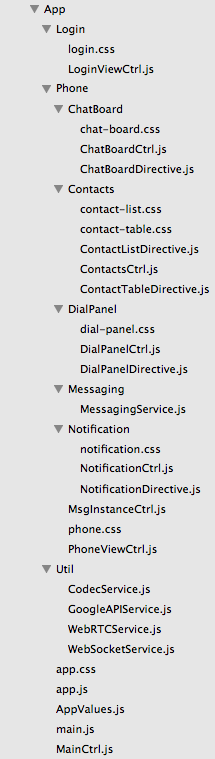
\includegraphics[height=0.45\textheight,natwidth=610,natheight=642]{figs/angularjs_structure.png}
  	\caption{Prototype Application AngularJs Files}
  	\label{fig:angularjs_structure}
\end{figure}

\end{appendices}